\documentclass[12pt,a4paper]{article}
% Fix for fancyhdr headheight error
\setlength{\headheight}{14.5pt}
% --- PACKAGES ---
% --- ENCODING & FONTS ---
\usepackage[utf8]{inputenc}
\usepackage[T1]{fontenc}
\usepackage{lmodern}          % Modern font (alternative to Times)
% \usepackage{times}          % OPTIONAL: Classic serif font (comment if using lmodern)

\usepackage{pgf-pie}
\usepackage{pgfplots}
\usepackage{subcaption}
\usepackage{xcolor}
\usepackage{colortbl}
\usepackage{multirow}
\usepackage{booktabs}
\usepackage{siunitx}
\usepackage{float}

% --- PAGE LAYOUT ---
\usepackage[a4paper, left=0.75in, right=0.75in, top=1in, bottom=1in]{geometry}
\usepackage{parskip}          % Paragraphs with spacing instead of indentation
\usepackage{setspace}         % For line spacing

% --- MATHEMATICS ---
\usepackage{amsmath, amsfonts, amssymb}

% --- GRAPHICS & FIGURES ---
\usepackage{graphicx}
\usepackage{caption}
\usepackage{float}
\usepackage{array, longtable, colortbl}
\usepackage{tabularx}

% --- COLORS ---
\usepackage[table]{xcolor}
\usepackage{xcolor}           % General color usage

% --- TIKZ & DIAGRAMS ---
\usepackage{tikz}
\usetikzlibrary{
  shapes.geometric,
  arrows.meta,
  positioning,
  fit,
  backgrounds,
  shapes.multipart
}

% --- PLOTS & CHARTS ---
\usepackage{pgf-pie}          % Pie charts
\usepackage{pgfplots}         % Graphs and plots
% Set pgfplots compatibility for modern features
\pgfplotsset{compat=1.18}

% --- DOCUMENT STRUCTURE ---
\usepackage{titlesec}         % Custom section titles
\usepackage{tocloft}          % Table of contents formatting
\usepackage{enumitem}         % Better lists

% --- HEADER, FOOTER & LINKS ---
\usepackage{fancyhdr}         % Custom headers/footers

% --- BIBLIOGRAPHY ---
\usepackage[numbers,sort&compress]{natbib}  % For references with numerical citations
\bibliographystyle{plainnat}  % Compatible style with natbib
\usepackage[many]{tcolorbox}
\tcbuselibrary{skins,breakable}

% --- Code listings for source code in Appendix ---
\usepackage{listings}
\lstset{
    language=Python,
    basicstyle=\ttfamily\small,
    breaklines=true,
    showstringspaces=false,
    numbers=left,
    numberstyle=\tiny\color{gray},
    frame=single,
    captionpos=b,
    keywordstyle=\color{blue},
    commentstyle=\color{green!60!black},
    stringstyle=\color{purple},
    rulecolor=\color{black!20},
    backgroundcolor=\color{black!5}
}

% --- Load hyperref last ---
\usepackage{hyperref}         % Clickable links


% --- COLORS ---
\definecolor{RoyalBlue}{RGB}{0, 70, 140}
\definecolor{RUETRed}{RGB}{179, 0, 0}
\definecolor{LightGray}{RGB}{248, 249, 250}
\definecolor{DarkGray}{RGB}{52, 58, 64}
\definecolor{AccentBlue}{RGB}{13, 110, 253}
\definecolor{ModernGray}{RGB}{108, 117, 125}
\definecolor{lightgreen}{RGB}{200, 255, 200}
\definecolor{lightred}{RGB}{255, 200, 200}

% Define modern color palette
\definecolor{primary}{RGB}{41, 128, 185}
\definecolor{secondary}{RGB}{52, 152, 219}
\definecolor{accent}{RGB}{231, 76, 60}
\definecolor{success}{RGB}{46, 204, 113}
\definecolor{warning}{RGB}{241, 196, 15}
\definecolor{darkgray}{RGB}{52, 73, 94}
\definecolor{lightgray}{RGB}{236, 240, 241}
\definecolor{purple}{RGB}{155, 89, 182}
\definecolor{orange}{RGB}{230, 126, 34}
\definecolor{teal}{RGB}{26, 188, 156}
\definecolor{OliveGreen}{RGB}{85, 107, 47}

\definecolor{outputbg}{RGB}{45, 45, 45} % Dark background for output

% --> ADDED for the blue info box
% --> Define colors for code boxes and result boxes
\definecolor{reportgreen}{RGB}{230, 245, 230}
\definecolor{reportdarkgreen}{RGB}{50, 120, 50}
\definecolor{outputbg}{RGB}{45, 45, 45} % Dark background for output
\definecolor{infoboxbg}{RGB}{235, 245, 255}
\definecolor{infoboxborder}{RGB}{70, 130, 180}
% --> ADDED: Define the blue info box style
\newtcolorbox{infobox}{
  colback=infoboxbg,
  colframe=infoboxborder,
  boxrule=0.5pt, % thin border for sides/bottom
  borderline north={1.5pt}{0pt}{infoboxborder}, % thicker top border
  arc=0mm,       % sharp corners
  left=5mm, % Add some padding
  top=3mm,
  bottom=3mm
}

% --> Define style for code listings (like Listing 2, 3 in friend's report)
\lstdefinestyle{code}{
    basicstyle=\ttfamily\small,
    numbers=left,
    numberstyle=\tiny\color{gray},
    numbersep=5pt,
    frame=none,
    breaklines=true,
    keywordstyle=\color{blue},
    commentstyle=\color{OliveGreen},
    stringstyle=\color{purple},
    showstringspaces=false
}
\lstset{style=code} % Set default listing style

% --> Define the green result box
\newtcolorbox{resultbox}[2][]{
    enhanced,
    attach boxed title to top center={yshift=-2mm},
    colback=reportgreen,
    colframe=reportdarkgreen,
    colbacktitle=reportgreen,
    coltitle=black,
    boxed title style={size=small,colframe=reportdarkgreen},
    title={#2},
    fonttitle=\bfseries
}

% --- FONT & STYLING ---
\renewcommand{\familydefault}{\sfdefault}  % Use sans-serif font
\titleformat{\section}{\fontsize{20}{24}\selectfont\bfseries\color{RoyalBlue}}{\thesection}{1em}{}
\titleformat{\subsection}{\fontsize{16}{20}\selectfont\bfseries\color{RoyalBlue}}{\thesubsection}{1em}{}
\titleformat{\subsubsection}{\fontsize{13}{16}\selectfont\bfseries\color{RoyalBlue}}{\thesubsubsection}{1em}{}

% TOC Styling
\renewcommand{\cfttoctitlefont}{\color{black}\Huge\bfseries}
\renewcommand{\cftsecfont}{\color{RoyalBlue}}
\renewcommand{\cftsecpagefont}{\color{RoyalBlue}}
\renewcommand{\cftsubsecfont}{\color{RoyalBlue}}
\renewcommand{\cftsubsecpagefont}{\color{RoyalBlue}}

% Header and Footer
\pagestyle{fancy}
\fancyhf{}
\fancyhead[C]{\textit{Digital Image Processing Report}}
\fancyfoot[C]{\thepage}
\renewcommand{\headrulewidth}{0.4pt}
\renewcommand{\footrulewidth}{0pt}

% Hyperlink Styling
\hypersetup{
    colorlinks=true,
    linkcolor=RoyalBlue,
    filecolor=magenta,
    urlcolor=cyan,
    pdftitle={Digital Image Processing Report},
    pdfpagemode=FullScreen,
    pdfborder={0 0 0},
}

% --- Define a global style for all plots for consistency ---
\pgfplotsset{
    every axis/.append style={
        axis x line=bottom,
        axis y line=left,
        label style={font=\bfseries},
        title style={font=\large\bfseries, yshift=1em},
        tick label style={font=\small},
        legend style={font=\small, at={(0.5,-0.2)}, anchor=north, legend columns=-1},
    }
}

% Modern title page with geometric design
\newcommand{\maketitlepage}{
    \begin{titlepage}
        \begin{tikzpicture}[remember picture,overlay]
            \fill[RoyalBlue!10] (current page.north west) rectangle ([yshift=-2.2cm]current page.north east);
            \fill[AccentBlue!5] ([yshift=-14cm]current page.north west) rectangle ([yshift=-16.2cm]current page.north east);
            \fill[RoyalBlue!15] ([xshift=2cm,yshift=-2cm]current page.north west) circle (1.2cm);
            \fill[AccentBlue!15] ([xshift=-2cm,yshift=-15.2cm]current page.north east) circle (0.9cm);
        \end{tikzpicture}

        \centering
        \vspace*{0.6cm}

        % Logo (only include if file exists)
        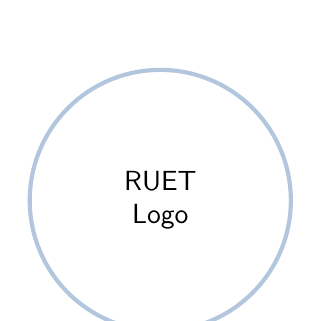
\begin{tikzpicture}
            \node[circle, draw=RoyalBlue!30, line width=1.5pt, inner sep=6pt] at (0,0) {
                 \IfFileExists{../RUET_logo.png}{\includegraphics[width=2.7cm]{../RUET_logo.png}}{\begin{minipage}{2.7cm}\centering RUET \\ Logo \end{minipage}}
            };
        \end{tikzpicture}

        \vspace{0.6cm}
        {\fontsize{15.5}{17}\selectfont\bfseries\textcolor{RUETRed}{RAJSHAHI UNIVERSITY OF ENGINEERING \& TECHNOLOGY}\par}
        \vspace{0.2cm}
        {\fontsize{13.5}{16}\selectfont\textcolor{DarkGray}{Department of Computer Science and Engineering}\par}

        \vspace{1.5cm}
        % Title Block
        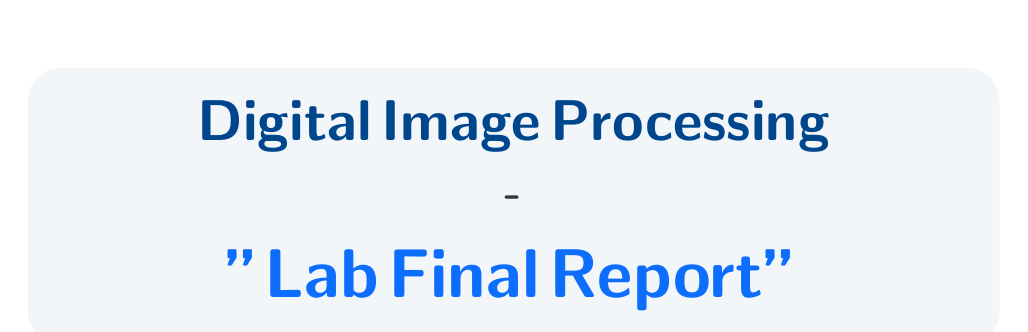
\begin{tikzpicture}
            \node[rectangle, fill=RoyalBlue!5, rounded corners=12pt, inner sep=12pt, text width=11.5cm, align=center] at (0,0) {
                {\fontsize{21}{24}\selectfont\bfseries\textcolor{RoyalBlue}{Digital Image Processing}\par}
                \vspace{0.15cm}
                {\fontsize{16}{20}\selectfont\bfseries\textcolor{DarkGray}{-}\par}
                \vspace{0.15cm}
                {\fontsize{24}{28}\selectfont\bfseries\textcolor{AccentBlue}{"Lab Final Report"}\par}
            };
        \end{tikzpicture}

        \vspace{1.8cm}
        % Submission info
        \begin{minipage}[t]{0.45\textwidth}
            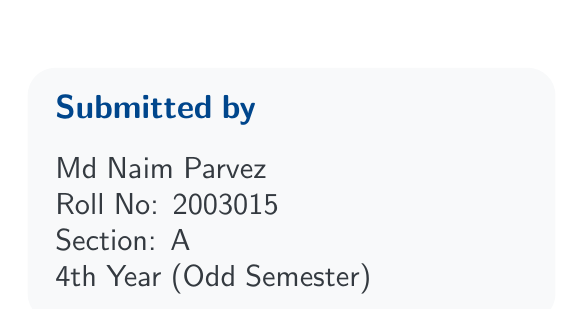
\begin{tikzpicture}
                \node[rectangle, fill=LightGray, rounded corners=10pt, inner sep=10pt, text width=6cm] at (0,0) {
                    {\fontsize{13}{15}\selectfont\bfseries\textcolor{RoyalBlue}{Submitted by}\par}
                    \vspace{0.3cm}
                    {\fontsize{11}{13}\selectfont\textcolor{DarkGray}{
                        Md Naim Parvez\\
                        Roll No: 2003015\\
                        Section: A\\
                        4th Year (Odd Semester)
                    }\par}
                };
            \end{tikzpicture}
        \end{minipage}
        \hfill
        \begin{minipage}[t]{0.50\textwidth}
            
\begin{tikzpicture}
                \node[rectangle, fill=AccentBlue!5, rounded corners=10pt, inner sep=10pt, text width=6cm] at (0,0) {
                    {\fontsize{13}{15}\selectfont\bfseries\textcolor{RoyalBlue}{Submitted to}\par}
                    \vspace{0.3cm}
                    {\fontsize{11}{13}\selectfont\textcolor{DarkGray}{
                        Utsha Das\\
                        Assistant Professor\\
                        Department of CSE\\
                        Rajshahi University of Engineering \& Technology\\
                        \vspace{0.3cm}
                    }\par}
                };
            \end{tikzpicture}
        \end{minipage}

        \vspace{1.2cm}
        % Course Info
        
\begin{tikzpicture}
            \node[rectangle, fill=RoyalBlue!10, rounded corners=10pt, inner sep=12pt, align=center, text width=13cm] at (0,0) {
                {\fontsize{13}{16}\selectfont\bfseries\textcolor{RoyalBlue}{Course Code: } \textcolor{DarkGray}{4106}}\\[0.2cm]
                {\fontsize{13}{16}\selectfont\bfseries\textcolor{RoyalBlue}{Course Title: } \textcolor{DarkGray}{Digital Image Processing Sessional}}
            };
        \end{tikzpicture}

        \vspace{0.8cm}
    \end{titlepage}
}


\begin{document}

% --- TITLE PAGE ---
\maketitlepage
\thispagestyle{empty} % No header/footer on the title page

% Abstract
\begin{abstract}
This project implements fundamental image processing techniques to enhance grayscale images. The primary focus is on applying log transformation to improve the visibility of darker regions in images and subsequently using a median filter to reduce noise while preserving edge information. The project demonstrates the implementation of these techniques from scratch using Python's modern scientific libraries: OpenCV, NumPy, and Matplotlib. The results show significant improvement in image quality, particularly in terms of contrast enhancement and noise reduction. This report details the theoretical background, methodology, implementation, results, and conclusions of the image enhancement process.
\end{abstract}

\newpage
% --- TABLE OF CONTENTS ---
\pagenumbering{roman} % Roman numerals for ToC, Abstract etc.
\phantomsection % Helps hyperref create proper links
\tableofcontents

% --- LIST OF FIGURES ---
\newpage
\phantomsection % Helps hyperref create proper links
\listoffigures
\newpage
\pagenumbering{arabic} % Arabic numerals for main content
\setcounter{page}{1} % Start main content page numbering from 1


%----------------------------------------------------------
% 1. Introduction
%----------------------------------------------------------
\section{Introduction}

\subsection{Motivation and Dataset Selection}

Road safety is a critical global concern, with traffic accidents ranking among the leading causes of injury and death worldwide. Identifying and predicting high-risk road conditions are essential steps toward designing smarter transportation systems and saving lives.  

For this project, the \textbf{Road Accident Risk Dataset} was selected. This synthetic dataset simulates real-world road conditions and represents a diverse range of environmental, infrastructural, and temporal variables. Its design supports predictive modeling tasks focused on estimating accident probabilities across different road segments.

\begin{infobox}{}
\textbf{Why Road Accident Risk Dataset?}
\begin{itemize}
    \item \textit{Real-World Context:} The dataset reflects the multidimensional nature of traffic safety—weather, lighting, surface type, and traffic density all interact to determine risk.
    \item \textit{Classification Feasibility:} By categorizing segments into low-, medium-, and high-risk classes, supervised learning algorithms can be effectively applied.
    \item \textit{Clustering Potential:} Numerical and categorical features allow for unsupervised exploration to uncover natural accident patterns.
    \item \textit{Data Challenge:} The dataset includes missing values and simulated anomalies, providing an opportunity to develop robust preprocessing pipelines.
\end{itemize}
\end{infobox}

\subsection{Dataset Characteristics and Noise Introduction}

The dataset consists of \textbf{1000 road segments} described by \textbf{10 attributes}, including environmental (e.g., lighting, weather), structural (e.g., number of lanes, curvature), and temporal variables (e.g., time of day, weekday vs. weekend). The target variable, \texttt{accident\_risk}, is a categorical label representing the probability of an accident.

\begin{resultbox}{}
\textbf{Noise Injection Strategy:}

\begin{itemize}
    \item \textit{Numeric Missing:} Randomly removed 2\% of entries from the \texttt{curvature} attribute.
    \item \textit{Categorical Missing:} Removed 3\% of entries from \texttt{weather}.
    \item \textit{Boolean Missing:} Removed 1\% of entries from \texttt{road\_signs\_present}.
    \item \textit{Integer Missing:} Removed 1\% of entries from \texttt{lighting}.
\end{itemize}
\end{resultbox}

Introducing noise intentionally strengthens the project’s realism. In real-world predictive systems, data imperfections are common. Handling them effectively ensures reliability when deploying models in operational settings like road monitoring or smart city dashboards.

\begin{figure}[H]
    \centering
    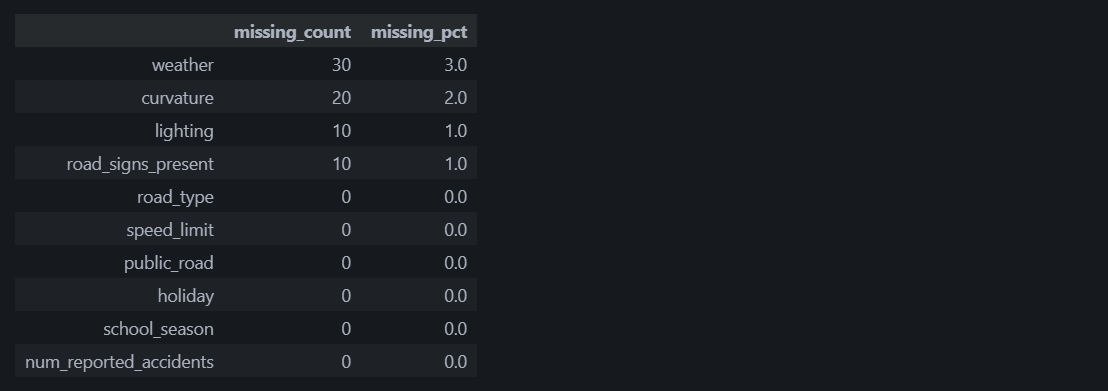
\includegraphics[width=0.8\textwidth]{missing_value.png}
    \caption{Visualization of noise introduction in different attributes of the dataset}
    \label{fig:noise_demonstration}
\end{figure}
\subsection{Lab Objectives and Task Overview}

The work follows a multi-stage data mining pipeline, composing tasks that transform raw data into actionable insights:

\begin{enumerate}
    \item \textit{Lab 1 – Dataset Analysis:}Understanding data structure, dimensions, and classification problem formulation. This initial step is crucial for identifying data types, detecting potential issues early, and determining the appropriate machine learning approach before investing time in modeling
    \item \textit{Lab 2 – Data Preprocessing:} Handling missing values, outliers, encoding, scaling, and similarity measures. Preprocessing is essential because algorithms cannot handle missing data or categorical variables directly, and unscaled features can bias distance-based methods.Quality input ensures quality output.
    \item \textit{Lab 3 – Exploratory Data Analysis (EDA):} Visualizing distributions, correlations, and patterns within the dataset. EDA provides insights into feature importance, class imbalances, and potential relationships that inform model selection and feature engineering strategies.
    \item \textit{Lab 4 – Mining Frequent Itemsets:} Applying Apriori algorithm to discover frequent patterns and association rules. Analysis of support, confidence, and lift metrics reveals purchase behaviors and product relationships. Understanding these patterns helps optimize inventory management and marketing strategies.
    \item \textit{Lab 5 – Classification:} Building Decision Tree models with entropy and Gini criteria.Classification transforms our understanding into actionable predictions, allowing us to automatically categorize fuel efficiency. Comparing criteria helps us select the optimal splitting strategy.
    \item \textit{Lab 6 – Clustering:} Applying k-Means and hierarchical clustering to discover natural groupings. Clustering uncovers hidden vehicle segments without predefined labels, validating our classification approach and revealing market structures that might inform manufacturing or marketing strategies.
\end{enumerate}

\begin{infobox}
\textbf{Why These Tasks Are Important:}
Each stage builds logically upon the previous one. Preprocessing ensures data quality; EDA uncovers structure and guides model selection; classification predicts accident risk levels; clustering validates hidden patterns. Together, they demonstrate how data-driven insights can translate into safer roads and informed infrastructure planning.
\end{infobox}

%----------------------------------------------------------
% 2. Dataset Deep Dive
%----------------------------------------------------------
\section{Dataset Deep Dive}

The Road Accident Risk dataset contains various attributes related to road conditions, vehicle characteristics, and environmental factors. Understanding these attributes is crucial for effective data analysis and model development.

\subsection{Attribute Breakdown}

The Road Accident Risk dataset contains the following key attributes:

- \textbf{road\_type:} Type of road (e.g., Highway, Urban, Rural)
- \textbf{curvature:} Measurement of road curvature
- \textbf{speed\_limit:} Posted speed limit
- \textbf{lighting:} Lighting conditions (Day, Night)
- \textbf{weather:} Weather conditions (Clear, Rain)
- \textbf{road\_signs\_present:} Presence of road signs
- \textbf{public\_road:} True if it is a public road
- \textbf{holiday:} True if the date is a public holiday
- \textbf{school\_season:} True if it is during school season
- \textbf{num\_reported\_accidents:} Count of previously reported accidents
- \textbf{accident\_risk:} Target variable (Low, Medium, High)

\begin{table}[H]
    \centering
    \sffamily % Use sans-serif font for tables
    \caption{Road Accident Risk Dataset Attributes}
    \label{tab:attributes}
    \begin{tabularx}{\textwidth}{l l X}
        \toprule
        \textbf{Feature} & \textbf{Type} & \textbf{Description} \\
    \midrule
    % --> Table content filled from your image
    road\_type & Categorical (object) & Type of road (e.g., Highway, Urban, Rural) \\
    \midrule
        curvature & Continuous (float64) & Measurement of road curvature \\
    \midrule
        speed\_limit & Discrete (int64) & Posted speed limit \\
    \midrule
        lighting & Categorical (object) & Lighting conditions (Day, Night) \\
    \midrule
        weather & Categorical (object) & Weather conditions (Clear, Rain) \\
    \midrule
        road\_signs\_present & Categorical (object) & Presence of road signs \\
    \midrule
        public\_road & Boolean (bool) & True if it is a public road \\
    \midrule
        holiday & Boolean (bool) & True if the date is a public holiday \\
    \midrule
        school\_season & Boolean (bool) & True if it is during school season \\
    \midrule
        num\_reported\_accidents & Discrete (int64) & Count of previously reported accidents \\
    \midrule
        accident\_risk & Categorical & \textbf{Target variable} (Low, Medium, High) \\
        \bottomrule
    \end{tabularx}
\end{table}

\subsection{Dataset Structure}

\begin{infobox}
\textbf{Dataset Overview:}
\begin{itemize}
    \item \textit{Total Instances:} 1000 rows, 10 columns
    \item \textit{Feature Space:} 9 independent variables
    \item \textit{Target Variable:} \texttt{accident\_risk} (categorical)
    \item \textit{Data Types:} Mix of Boolean, discrete (int64), and categorical (object/category)
    \item \textit{Split Strategy:} 80\% training (800 samples), 20\% test (200 samples)
\end{itemize}
\end{infobox}

\begin{figure}[H]
    \centering
    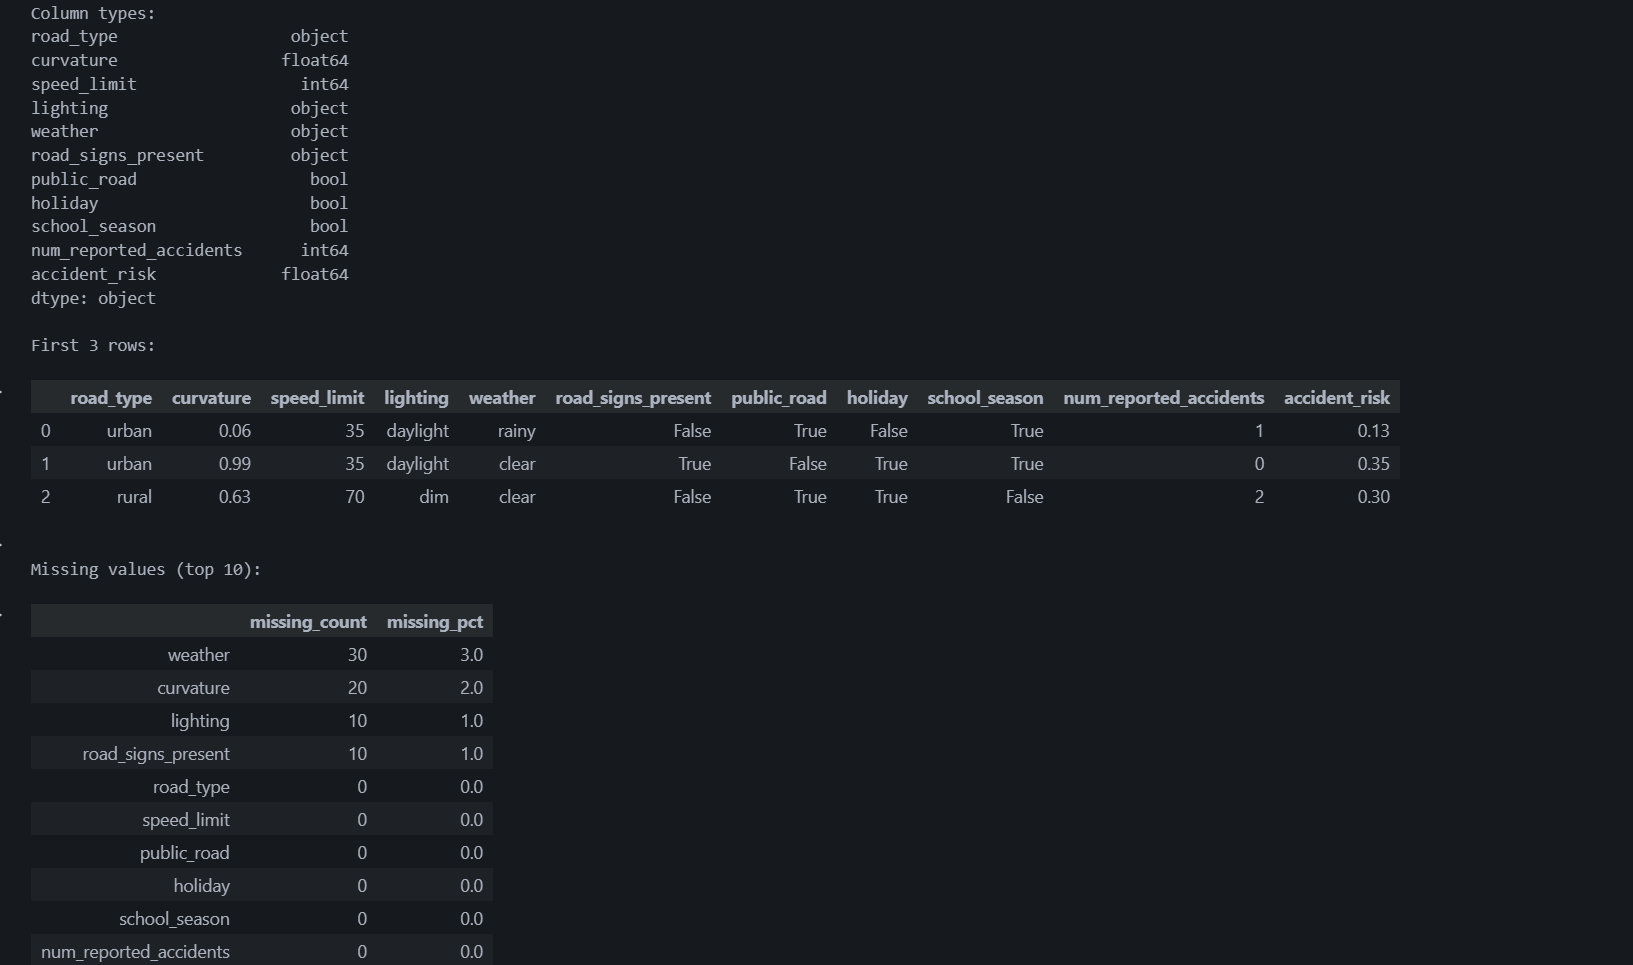
\includegraphics[width=1\textwidth]{df_structure.png}
    \caption{Dataset structure and basic information overview}
    \label{fig:dataset_structure}
\end{figure}


\subsection{Problem Formulation: Multiclass Classification}

The road accident risk prediction problem is formulated as a \textbf{multiclass classification task}, where we aim to predict the categorical risk level of road segments based on their environmental, structural, and temporal characteristics.

\subsubsection{Class Distribution and Balance}

Understanding the target variable distribution is crucial for selecting appropriate evaluation metrics and handling potential class imbalance issues.

\begin{resultbox}{}
\textbf{Class Distribution Analysis:}
The dataset exhibits a relatively balanced distribution across risk categories:
\begin{itemize}
    \item \textbf{Low Risk:} Approximately 34.5\% of road segments
    \item \textbf{Medium Risk:} Approximately 33.3\% of road segments  
    \item \textbf{High Risk:} Approximately 32.2\% of road segments
\end{itemize}
This balanced distribution is advantageous as it reduces the need for specialized sampling techniques and allows standard classification metrics to be meaningful across all classes.
\end{resultbox}

\begin{figure}[H]
    \centering
    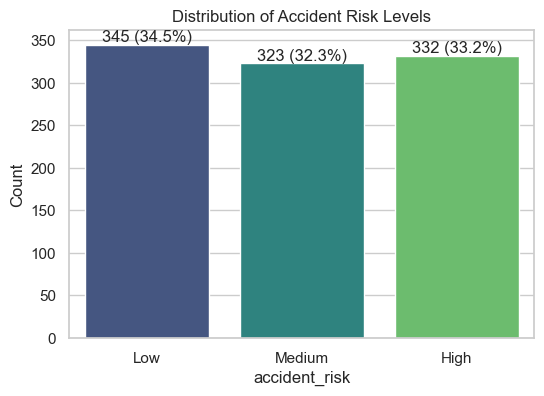
\includegraphics[width=0.7\textwidth]{Distribution.png}
    \caption{Distribution of accident risk levels in the dataset}
    \label{fig:class_distribution}
\end{figure}

\subsubsection{Feature Space Characteristics}

The feature space combines multiple data types that require different preprocessing approaches:

\begin{table}[H]
    \centering
    \sffamily
    \caption{Feature categorization for preprocessing strategy}
    \label{tab:feature_types}
    \begin{tabularx}{\textwidth}{l l X}
        \toprule
        \textbf{Category} & \textbf{Features} & \textbf{Preprocessing Required} \\
        \midrule
        Numerical & curvature, speed\_limit, num\_reported\_accidents & Scaling, outlier detection \\
        \midrule
        Categorical & road\_type, lighting, weather, road\_signs\_present & Encoding (One-hot/Label) \\
        \midrule
        Boolean & public\_road, holiday, school\_season & Binary encoding (0/1) \\
        \bottomrule
    \end{tabularx}
\end{table}

\subsubsection{Classification Challenges}

Several challenges make this classification problem non-trivial:

\begin{enumerate}
    \item \textbf{Mixed Data Types:} The combination of numerical, categorical, and boolean features requires careful preprocessing to maintain information integrity.
    
    \item \textbf{Missing Values:} Artificially introduced noise simulates real-world data imperfections that must be handled appropriately.
    
    \item \textbf{Feature Interactions:} Road safety is influenced by complex interactions between environmental factors (weather × lighting), temporal factors (holiday × school\_season), and infrastructure characteristics.
    
    \item \textbf{Non-linear Relationships:} The relationship between features and accident risk may be non-linear, requiring sophisticated algorithms or feature engineering.
\end{enumerate}

\section{Methodology and Implementation}

\subsection{Dataset Analysis}

This initial phase focused on understanding the dataset structure, loading the data, and preparing it for subsequent analysis tasks.

\subsubsection{Data Loading and Initial Inspection}

The original Road Accident Risk Dataset contains over 500,000 samples, which presents computational challenges for analysis and model training. To ensure efficient processing while maintaining statistical representativeness, we implemented a systematic sampling approach that selects the first 1,000 samples for our analysis.

\begin{resultbox}{Dataset Loading Strategy}
\textbf{Sampling Justification:}
\begin{itemize}
    \item \textit{Computational Efficiency:} 1,000 samples provide sufficient data for meaningful analysis while ensuring reasonable processing times
    \item \textit{Prototype Development:} Enables rapid iteration and model development before scaling to larger datasets
\end{itemize}
\end{resultbox}

\begin{lstlisting}[language=Python, caption=Dataset Loading and Initial Sampling, label=lst:dataset_loading]
df_train = pd.read_csv('train.csv')
print(df_train.shape)
# Output: (517754, 14)
df_train.drop(['id','num_lanes','time_of_day'],axis=1,inplace=True)
df_train_sample = df_train.head(1000).copy()
print(df_train_sample.shape)
#output:df_train_sample shape: (1000, 11)

\end{lstlisting}

The sampling approach ensures we have a manageable yet representative subset of the original dataset. This 1,000-sample dataset maintains the essential characteristics of the full dataset while enabling efficient exploration, preprocessing, and model development.

\subsection{Adding Missing value:}
To simulate real-world data imperfections, we intentionally introduced missing values into specific attributes of the dataset. This process involved randomly removing a certain percentage of entries from selected features, thereby creating a more challenging and realistic dataset for analysis.
\begin{lstlisting}[language=Python, caption=Introducing Missing Values into the Dataset, label=lst:missing_value_injection]
# create copies so original dfs remain available
df_train_missing = df_train.copy()
df_train_sample_missing = df_train_sample.copy()

# reproducible random selection
rng = np.random.RandomState(42)

missing_config = {
    'curvature': 0.02,           # 2% missing (numeric)
    'lighting': 0.05,            # 5% missing (categorical)
    'weather': 0.03,             # 3% missing (categorical)
    'road_signs_present': 0.01,  # 1% missing (boolean -> will become object/float after NaN)
    'lighting': 0.01,           # 1% missing (integer)
}

# helper to inject missing values into a dataframe
def inject_missing(df, config, rng):
    n_rows = len(df)
    for col, frac in config.items():
        n_missing = int(np.floor(frac * n_rows))
        if n_missing <= 0:
            continue
        idx = rng.choice(df.index, size=n_missing, replace=False)
        df.loc[idx, col] = np.nan
    return df

df_train_sample_missing = inject_missing(df_train_sample_missing, missing_config, np.random.RandomState(7))
print("\nMissing counts in df_train_sample_missing:")
print(df_train_sample_missing.isnull().sum())

\end{lstlisting}

\begin{figure}[H]
    \centering
    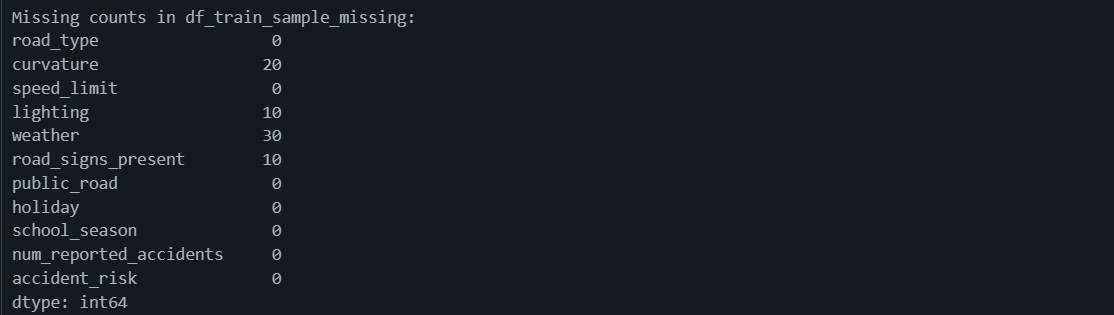
\includegraphics[width=0.8\textwidth]{add_missing_value.png}
    \caption{Missing value injection results}
    \label{fig:missing_values_injection}
\end{figure}

\subsection{EDA :}
    Exploratory Data Analysis (EDA) was conducted on the dataset to uncover patterns, trends, and relationships within the data. This process involved visualizing the distribution of key features, examining correlations, and identifying potential anomalies or outliers.

    \begin{itemize}
        \item \textbf{Feature Distributions:} Histograms and bar plots were created to visualize the distribution of numerical and categorical features, respectively. This helped identify skewness, modality, and potential outliers.
        \begin{lstlisting}[language=Python, caption=Exploratory Data Analysis (EDA) Implementation, label=lst:eda_implementation]
       # Plot numerical columns in a single row
       numerical_cols = ['curvature', 'speed_limit', 'num_reported_accidents']
       n = len(numerical_cols)
       fig, axes = plt.subplots(1, n, figsize=(5 * n, 5))
       # Ensure axes is iterable
       axes = np.atleast_1d(axes)

      for i, col in enumerate(numerical_cols):
        sns.histplot(df_train_sample_missing[col], bins=30, kde=True, ax=axes[i])
        axes[i].set_title(f'Distribution of {col}')
        axes[i].set_xlabel(col)
        axes[i].set_ylabel('Count')

    plt.tight_layout()
    plt.show()
        \end{lstlisting}
    \begin{lstlisting}[language=Python, caption=Categorical Feature Distribution Visualization, label=lst:categorical_feature_distribution]
    # Plot categorical columns in a single row
    categorical_cols = ['road_type', 'lighting', 'weather', 'road_signs_present']
    n = len(categorical_cols)
    fig, axes = plt.subplots(1, n, figsize=(5 * n, 5))
    # Ensure axes is iterable
    axes = np.atleast_1d(axes)

    for i, col in enumerate(categorical_cols):
        sns.countplot(x=df_train_sample_missing[col], ax=axes[i])
        axes[i].set_title(f'Distribution of {col}')
        axes[i].set_xlabel(col)
        axes[i].set_ylabel('Count')

    plt.tight_layout()
    plt.show()
    \end{lstlisting}
        \begin{figure}[H]
            \centering
            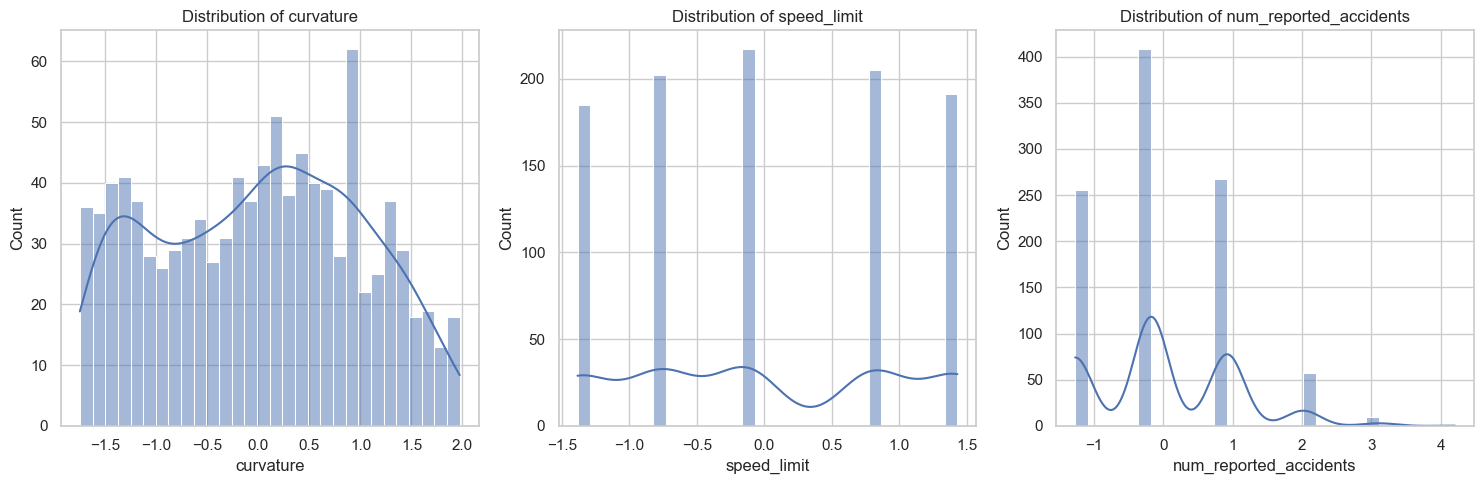
\includegraphics[width=1\textwidth]{numerical_density.png}
            \caption{Feature distributions of key attributes(Numerical)}
            \label{fig:feature_distributions}
        \end{figure}
    \textbf{Findings from Numerical Distributions:}
\begin{itemize}
    \item \textit{curvature:} The distribution is heavily right-skewed, with the vast majority of road segments having very low curvature (close to 0).
    \item \textit{num\_reported\_accidents:} This is a discrete variable, with a decreasing frequency as the number of accidents increases.
    \item \textit{speed\_limit:} This plot clearly shows distinct, discrete peaks corresponding to standard speed limits (e.g., 35, 45, 60, 70 mph/kph).
\end{itemize}
        \begin{figure}[H]
            \centering
            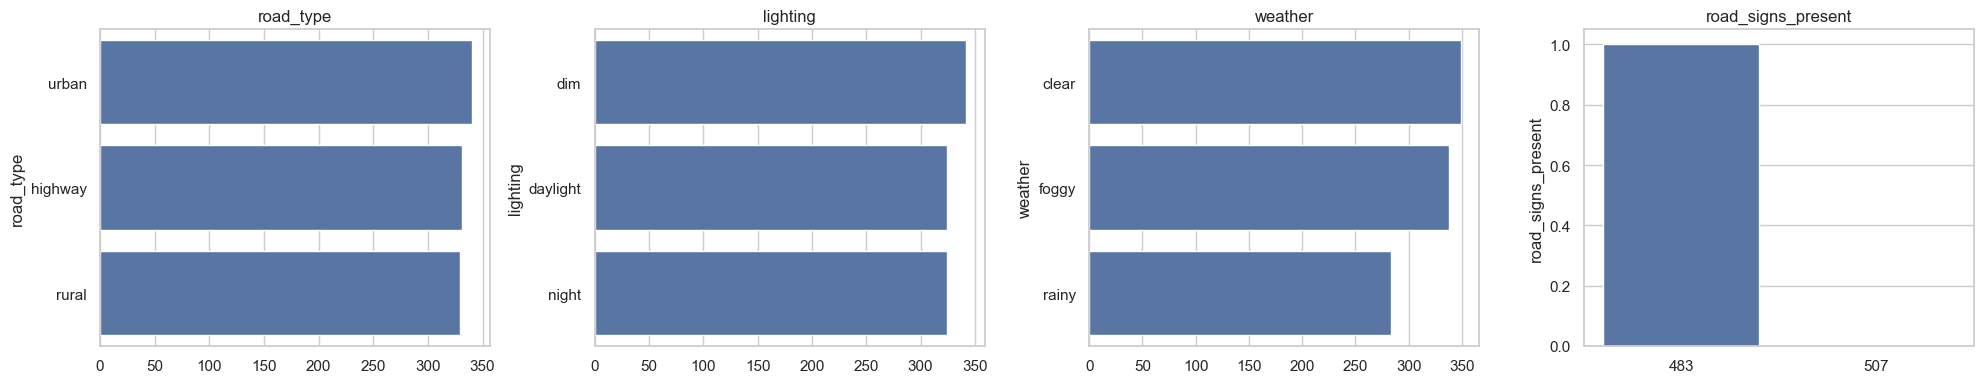
\includegraphics[width=1\textwidth]{category_bool.png}
            \caption{Feature distributions of key attributes(Categorical)}
            \label{fig:feature_distributions_categorical}
        \end{figure}
    \end{itemize}
    \textbf{Findings from Categorical Distributions:}
\begin{itemize}
    \item \textit{road\_type:} The dataset contains three types, with 'urban' being the most frequent, followed by 'highway' and 'rural'.
    \item \textit{lighting \& weather:} For lighting, 'daylight' is the most common condition. For weather, 'clear' is the most common.
    % --> ERROR FIX: Escaped the underscores in the line below
    \item \textit{Boolean Features:} The boolean plots show the balance of \texttt{public\_road} (mostly True), \texttt{holiday} (mostly False), \texttt{school\_season} (roughly balanced), and \texttt{road\_signs\_present} (roughly balanced).
\end{itemize}
    
\end{document}

